\documentclass[12pt]{article}
\usepackage[margin=1in]{geometry}
\usepackage{hyperref}
\usepackage{subcaption}
\usepackage{graphicx}

\setlength\parskip{5mm}
\widowpenalty10000
\clubpenalty10000
\setlength\parindent{0pt}

\begin{document}

\section{Introduction}

Boundary Value problems history and motivation

Types of boundaries

\section{Procedure}

Discreetizing Poisson equation

Solving discreet poisson eq.
 - Jacobi
 - SOR

Overview of program design

Determining when to halt

Motivation for correctness checks

Correctness Checks
 - Solution to sin(x) along wall potential -- non-discreet.
 - Electric dipole solution for far away

Calculating correctness automatically

Computer performance measurements and program optimization concerns
 - General Thoughts (use C)
 - Caching
 - Threading
 - SIMD

\section{Results}

Results of sin(x)

Result of dipole (compare to monopole)

Performance Results

\section{Conclusion}

Future Work



\clearpage
\section{Appendix A - Program Usage}

Compiling the engine (the C library) requires make and gcc (or clang, though clang is untested), and can
be done by simply invoking \texttt{make}. This will also create an executable file, \texttt{solve}. This
is a script that invokes the python example frontend so that it may be used.

For more details on using the python frontend or the C backend engine, see the man pages (reproduced on the
following pages). There are several example files, including \texttt{example\_sin.txt} and \texttt{example\_dipole.txt}.
For more details on writing configurations for a desired simulation or experiment, see the man pages.

The source code also contains a directory named \texttt{tests}, which contains python code to generate verifier data
files for the \texttt{example\_sin} configuration. Finally, all of the data written on in this document are present
in the source directory, under \texttt{results}. The source code for the C library is in \texttt{engine}, and the
source code for the python example frontend is under \texttt{frontend}. The source code and git revision history
is available at \url{http://github.com/dbittman/statics-solver}.

\begin{flushleft}
	SOLVE(1)
	\hfill User Commands \hfill
	SOLVE(1)
\end{flushleft}

\begin{tabbing}
\hspace{30pt}\=\hspace{30pt}\=\kill

\textbf{NAME}\\
\> solve - Solve Discreet Poisson Equation\\
\\
\textbf{SYNOPSIS}\\
	\> \texttt{solve [-V] [-m \textit{method}] [-v \textit{verification-data}] \textit{configuration-file}}\\
	\\
\textbf{DESCRIPTION}\\
\> Solve Poisson Equation given boundary conditions on a discreet grid. Capable of\\
\> solving physics problems that reduce to a boundary value problem. Operates on the\\
\> provided configuration file, producing a 2-D array describing the calculated potential.\\
\\
\> \texttt{\textbf{-V}} \\
\> \> Produce a vector plot, where the vectors are the negative gradient of the potential.\\
\\
	\> \texttt{\textbf{-m} \textit{method}} \\
	\> \> Use method \textit{method} when solving. Current supported values are \texttt{jacobi} for\\
	\> \> Jacobi Iteration, and \texttt{sor} for Successive Over-Relaxation.\\
\\
	\> \texttt{\textbf{-v} \textit{verification-data}} \\
	\> \> Use the data file \textit{verification-data} to compare with the generated potential. The \\
	\> \> format for this file must be that of the python library pickle serializing a 2-D array.\\
\\
\textbf{CONFIGURATION}\\
\> The configuration file format is specified by a series of commands on lines. A single line\\
\> can contain at most one command. A command must be contained within one line.\\
\> Comments begin with a \#, and comment out the rest of that line. Valid commands are\\
\> as follows, where italics indicates something to be replaced by one token:\\
\\
	\> \texttt{gridsize \textit{size}}\\
	\> \> Set the size of the grid. The grid is always a square, and this command \textbf{must}\\
	\> \> come before any other.\\
	\\
	\> \texttt{cell \textit{coords} initial \textit{value}}\\
	\> \> Specify initial value of a cell inside the grid. Analogous to a point charge.\\
	\\
	\> \texttt{dirichlet \textit{coords} \textit{coords} = \textit{value}}\\
	\> \> Specify a diriclet boundary condition along the interpolated straight line from the\\
	\> \> first set of coordinates to the second with value \textit{value}.\\
\end{tabbing}
\begin{flushleft}
	statics-solver
	\hfill March 2016 \hfill
	SOLVE(1)
\end{flushleft}
\clearpage
\begin{flushleft}
	SOLVE(1)
	\hfill User Commands \hfill
	SOLVE(1)
\end{flushleft}

\begin{tabbing}
\hspace{30pt}\=\hspace{30pt}\=\kill
	\> \texttt{neumann \textit{coords} \textit{coords} \textit{direction} = \textit{value}}\\
	\> \> Specify a diriclet boundary condition along the interpolated straight line from the\\
	\> \> first set of coordinates to the second with value \textit{value} across the boundary of the\\
	\> \> cells specified by \textit{direction}, which may be one of \texttt{left, up, right, down}.\\
	\\
	\> The values of \texttt{\textit{coords, size, direction}} must all be one token, that is,\\
	\> they may not contain any whitespace. The contents of \texttt{\textit{value}} and \texttt{\textit{coords}} are\\
	\> as follows:\\
	\\
	\> \texttt{\textit{value}} is an \texttt{expression}.\\
	\\
	\> \texttt{\textit{coords}} is an \texttt{expression} followed by a comma, followed by an \texttt{expression}.\\
	\\
	An \texttt{expression} is a valid python expression, with access to the python math library, the\\
	current grid class, and the current position in the grid as specified by \texttt{x} and \texttt{y}. For \\
	example, \texttt{math.sin(x*math.pi/grid.len)} is a valid \texttt{expression}.\\
	\\
	\textbf{AUTHOR}\\
	\> Written by Daniel Bittman (\texttt{danielbittman1@gmail.com}). Please submit any bug\\
	\> reports to this email address.\\
	\\
	\textbf{COPYRIGHT}\\
	\> Copyright\copyright Daniel Bittman. License MIT software license. This is free software, and\\
	\> is provided with NO WARRANTY.\\
	\\

\end{tabbing}
\begin{flushleft}
	statics-solver
	\hfill March 2016 \hfill
	SOLVE(1)
\end{flushleft}


\begin{flushleft}
	SOLVER(3)
	\hfill Libraries \hfill
	SOLVER(3)
\end{flushleft}

\begin{tabbing}
\hspace{30pt}\=\hspace{30pt}\=\kill

\textbf{NAME}\\
\> solver - Library to solve Discreet Poisson Equation\\
\\
\textbf{SYNOPSIS}\\
	\> \texttt{solver.h}\\
	\> \> \texttt{SOLVE\_METHOD\_JACOBI}\\
	\> \> \texttt{SOLVE\_METHOD\_SOR}\\
	\> \texttt{double \textbf{solve}(struct grid *grid, int method);}\\
	\> \texttt{void \textbf{init\_grid}(struct grid *grid);}\\
	\> \texttt{struct grid \{}\\
	\> \> \texttt{int len;}\\
	\> \> \texttt{int iters;}\\
	\> \> \texttt{float **values;}\\
	\> \> \texttt{float **value\_prevs;}\\
	\> \> \texttt{float **initials;}\\
	\> \> \texttt{uint8\_t **dirichlet\_presents;}\\
	\> \> \texttt{float **dirichlets;}\\
	\> \> \texttt{uint8\_t **neumann\_presents;}\\
	\> \> \texttt{float **neumanns[4];}\\
	\>\texttt{\};}\\
\\
\textbf{DESCRIPTION}\\
\> This library provides fast solving of a 2-D discreet boundary value problem using the\\
	\> Poisson equation. The full process is to define a \texttt{struct grid}, and set its \texttt{len} field. Then\\
	\> call \texttt{init\_grid} on the grid to initialize the 2-D contiguous arrays. After that, call \texttt{solve}\\
	\> and pass it the grid and a method, either \texttt{SOLVE\_METHOD\_JACOBI} or \texttt{SOLVE\_METHOD\_SOR}.\\
	\\
	\> The \texttt{solve} function will return when complete, returning back a value describing how\\
	\> confident it is in its result (values closer to zero are better). The \texttt{iters} field in the grid\\
	\> will have been updated to indicate how many iterations the program took. The \texttt{values}\\
	\> field points to a 2-D array of size \texttt{len} by \texttt{len} containing the solution.\\
	\\
	\textbf{AUTHOR}\\
	\> Written by Daniel Bittman (\texttt{danielbittman1@gmail.com}). Please submit any bug\\
	\> reports to this email address.\\
	\\
	\textbf{COPYRIGHT}\\
	\> Copyright\copyright Daniel Bittman. License MIT software license. This is free software, and\\
	\> is provided with NO WARRANTY.\\
	\\

\end{tabbing}
\begin{flushleft}
	statics-solver
	\hfill March 2016 \hfill
	SOLVER(3)
\end{flushleft}


\clearpage

\section{Appendix B - Computer Program Optimization}

When optimizing a program, there is an important cardinal rule to follow which at times
is easy to forget in the face of increasingly interesting and complex minor optimizations
designed to squeeze every bit of performance out of your computer. Unfortunately, due
to the complexity of modern computer hardware, it is
very difficult to predict if a given micro-optimization will actually be benificial or
not. For this reason, the most important rule when taking a working program and making it
fast is\footnote{besides \textit{don't break it}, of course. An incorrect program is worthless, no matter
how fast it is.} \textit{benchmark everything}.

The field of program optimization is huge. There is a small number of people who, for
a given platform, are really \textit{good} at optimization. There is an even smaller number
who are truly experts. I do not fit into either of these categories. For this reason, the program
that I have written here is \textit{decently} optimized. I believe that the maximum throughput
is not orders of magnitude better than what I have achieved, however, there is still a lot of work
that can be done (including a potentially significant optimization that I have neglected, and will talk
about later).

%%%%%%%%%%%%%%%%%%%%%%%%%%%%%%%%%%%%%%%%%% ACTUALLY TALK ABOUT THAT ************************

\subsection{Freebies}

There are some optimizations which can be used in high confidence and are also very easy to do.
The first, and most obvious, is to use a fast language. While writing in \texttt{C} may be a chore
compared to writing in python, the resulting code will be much faster. This is the reason behind the
organization of this program: the frontend (which has no performance requirements) is written in
python because parsing the configuration file is much easier. The backend needs to be fast, so it
is implemented in \texttt{C}.

A quick and rough experiement can easily convince you that this is true (remember how I said to
benchmark everything?). Credit to my friend Chris Milke for doing this test. Write the following
code in both python and in C: initialize a variable to zero. Then loop from zero to some large
number (we used 123,456,789), and add that iteration to the variable. After the loop, print the
variable. The resultant python program took 14.25 seconds to run on my computer, but the C code
completed \textit{instantaneously}. Why is python slower than C in general? Because python is
an interpreted language. The code that you write is read by another program and executed by
that program. In contrast, C code must be compiled into machine code. This is then run directly
on the processor, which cuts out the middle-man of the interpreter.

When using C, there are some more things that you can get for free: compiler optimizations. When
compiling a C program, the command looks something like this: \texttt{gcc -Wall -Wextra foo.c}\footnote{as an aside, you should \textbf{always} compile with -Wall and -Wextra, and eliminate all warnings from your program.
Warnings are warnings for a reason, and should rarely be ignored.}. This will
result in a compiled C program (a binary file, containing the machine code), but it will be
unoptimized. There are reasons why one may want an unoptimized binary (they are typically
easier to debug, for example), but generally when you compile your program for actual usage
you will want to optimize it. An aggressive optimization compilation command may look something
like: \texttt{gcc -Wall -Wextra -O3 -ffast-math -mavx}, as a start. The main flag here is \texttt{-O3}, which
enables almost every optimization that gcc can do.

Going back to the example from earlier, the optimized version of the C program completed instantly, but
the unoptimized version took 0.33 seconds. The unoptimized version is still 43 times faster than the
python code, but what was the optimizing compiler doing to make it so much faster with \texttt{-O3} on?
Part of optimizing is understanding why something is faster, so lets look at the assembly code. On \textsc{unix},
this can be done with the objdump command. Table \ref{table:assem-1} shows the annotated assembly from
the function \texttt{main}. If you don't know x86\_64 assembly language, you will at least notice that the
optimized version is much shorter. If you do know how to read the assembly, you'll notice that the unoptimized
version is doing almost literally what the C code says to do: set a variable to zero, and iterate from zero to
a big number, adding that iteration to the variable, and finally printing the variable. The optimized code just prints a large number -- which happens to be the result of the sum.

\begin{table}[h]
	\centering
\begin{tabular}{l | l}
	\hline
	\textbf{Unoptimized} & \textbf{Optimized}\\
	\hline
	\texttt{mov [rbp-0x10], 0x0}	&\texttt{movabs rsi,0x1b131147ee6b52} \\
	\texttt{jmp .loop\_end			}	&\texttt{mov edi,0x400594} \\
	\texttt{.loop\_top:                } &\texttt{xor eax,eax   } \\
	\texttt{mov rax, [rbp-0x10]				}	&\texttt{jmp 4003c0 <printf@plt>}\\
	\texttt{add [rbp-0x8], rax				}	&\texttt{	} \\
	\texttt{add [rbp-0x10], 0x1				}	&\texttt{ }\\	
	\texttt{.loop\_end:                       } &\texttt{} \\
	\texttt{cmp [rbp-0x10],0x75bcd14} &\texttt{} \\
	\texttt{jle loop\_top} &\texttt{} \\
	\texttt{mov rsi,[rbp-0x8]} &\texttt{} \\
	\texttt{mov edi, 0x4005b4} &\texttt{} \\
	\texttt{mov eax, 0} &\texttt{} \\
	\texttt{call 4003c0 <printf@plt>} &\texttt{} \\
\end{tabular}
	\caption{Unoptimzed and optimized assembly from the sum-a-lot-of-numbers example.}
	\label{table:assem-1}
\end{table}

This is just a simple example, but a good C compiler can drastically improve the performance of a
program. Here, it made a program that took a third of a second (which is already drastically faster than
the interpreted python version!) finish instantly.

\subsection{A Model of Processor Design}



\begin{figure}[h]
\begin{subfigure}{0.4\textwidth}
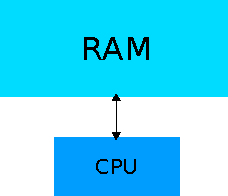
\includegraphics[width=\linewidth]{ram-cpu-simple.pdf}
\caption{Simplistic view of CPU and RAM.} \label{fig:1a}
\end{subfigure}
\hfill
\begin{subfigure}{0.4\textwidth}
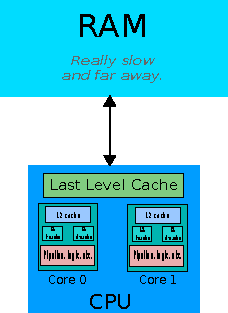
\includegraphics[width=\linewidth]{ram-cpu-complex.pdf}
\caption{More realistic view of CPU and RAM.} \label{fig:1b}
\end{subfigure}
\label{fig:cpu-and-ram}
\caption{View of programming that programmers like to have (a), versus the the more realistic
and complicated view.}
\end{figure}


\subsection{Structure of Arrays}

\subsection{Multithreading}

\subsection{Vectorization}
\subsubsection{Branch Reduction}



\section{Appendix C - Program Implementation}


\end{document}

